\chapter{Proposed Approach}
\label{chap:system}
\setlength{\parskip}{1.5mm}
%\setlength{\baselineskip}{1.4mm}
The proposed algorithm of encryption \& decryption is based on multiple iterations of a certain dynamical chaotic system and using a Baptista-type encryption-decryption scheme from the chaotic map generated. After referring extensive literature and keeping in mind the resources at our disposal, we have decided to take the compound triple-pendulum model for creating the chaotic map in our cryptosystem. We assume that input to the system is a plain message. The system parameter(s) and additionally the initial conditions of the dynamical system are assumed to be the part of the secret key. After simulating the triple-pendulum, our next step would be to generate a valid set of keys for encryption and decryption. The entire mechanical model would then be implemented on {\em Artix FPGA} including the design and implementation of ALU and Control Unit, adhering to the performance specification of the problem. Additionally, an extra data transfer module can be added to the hardware for key exchanges.\\
The entire approach can be summarized using the following roadmap :- 
\begin{figure}[H]
\vfill
\tikzstyle{startstop} = [rectangle, rounded corners, minimum width=3cm, minimum height=0.8cm,text centered, draw=black, fill=orange!30]
\hspace{1.8cm}
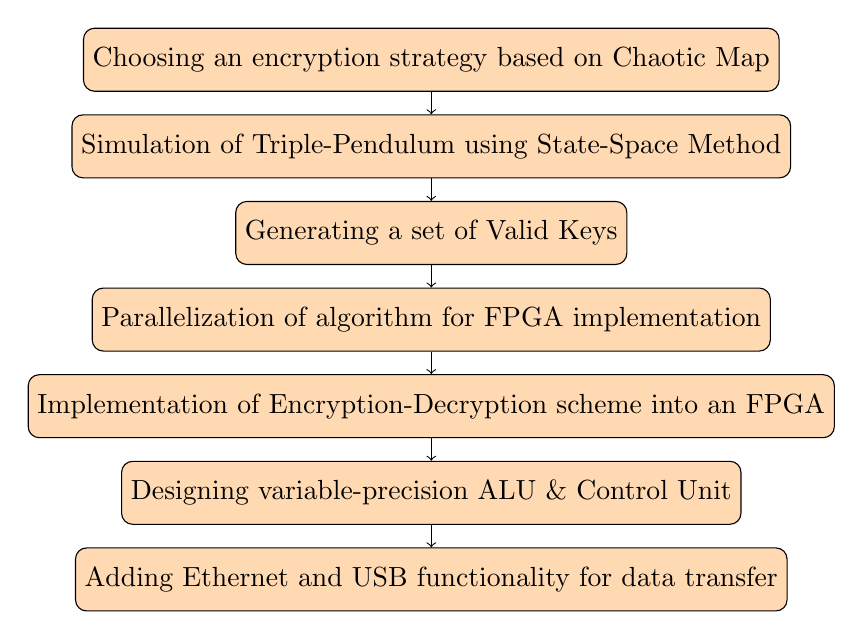
\begin{tikzpicture}[node distance=1.1cm]

\node (block1) [startstop, yshift=-4cm] {Choosing an encryption strategy based on Chaotic Map};

\node (block2) [startstop, below of=block1] {Simulation of Triple-Pendulum using State-Space Method};

\node (block3) [startstop, below of=block2] {Generating a set of Valid Keys};

\node (block4) [startstop, below of=block3] {Parallelization of algorithm for FPGA implementation};

\node (block5) [startstop, below of=block4] {Implementation of Encryption-Decryption scheme into an FPGA};

\node (block6) [startstop, below of=block5] {Designing variable-precision ALU \& Control Unit};

\node (block7) [startstop, below of=block6] {Adding Ethernet and USB functionality for data transfer};

\draw [->] (block1) -- (block2);
\draw [->] (block2) -- (block3);
\draw [->] (block3) -- (block4);
\draw [->] (block4) -- (block5);
\draw [->] (block5) -- (block6);
\draw [->] (block6) -- (block7);
\end{tikzpicture}
\vfill
\caption{Implementation Steps}
\end{figure}
